In this section, we present our program analysis {\THESYSTEM} for
computing an upper bound on the \emph{adaptivity} of a given program
$c$.  The high level idea behind {\THESYSTEM} is to first build
an \emph{estimated dependency graph} \progG(c) of a program $c$
(Section~\ref{sec:alg_weightedgegen}) which overapproximates the
semantics-based dependency graph in two dimensions: it
overapproximates the dependencies between assigned variables (Section~\ref{sec:alg_edgegen}), and, it
overapproximates the weights (Section~\ref{sec:alg_weightgen}). Then, {\THESYSTEM} uses a custom algorithm to estimate the longest
walk on this graph, providing in this way an upper bound on the adaptivity of the
program.



%%   \item \textbf{Edge and Weight Estimation} in Section~\ref{sec:alg_weightedgegen}. It combines the dependency analysis and quantitative analysis techniques in three steps as follows,
%% %   the control, data-flow  analysis algorithm and the loop bound inference algorithm.
%% %   There are three computation steps in this algorithm.
%%   \\
%% %   \textbf{1. Abstract Control Flow Graph.}
%%   a. In order to perform these combined analysis techniques, Section~\ref{sec:abscfg} first generates an \emph{abstract control flow graph}, $\absG(c)$ for the program $c$.
%%   \\
%%   b. Section~\ref{sec:alg_edgegen} estimates the edges of $\traceG(c)$
%% %   It performs over 
%%   based on the \emph{abstract control flow graph}, and combines the control flow and data flow analysis techniques.
%%   It estimates our \emph{variable may-dependency} between each pair of the labeled variables in a program by considering both the control flow and data flow,
%% %   Then it uses the estimated dependency relation to approximate the edge
%% %   between each pair of vertices.
%% and use it to estimate the edge.
%%   \\
%%   c. Section~\ref{sec:alg_weightgen} estimates the weight of $\traceG(c)$
%% %   It performs over the same \emph{abstract control flow graph}, 
%% based on the same $\absG(c)$
%% % and computes the upper bound on the maximal visiting times of each labeled variable for a program.
%%   It estimates the reachability bounds on the maximal visiting times for $\absG(c)$'s vertices ,
%%   and use them to estimate the bound on the visiting time of $x^l \in \lvar(c)$ and its weight.
%% \item  Section~\ref{sec:alg_graphgen} constructs the final approximated graph,
%% named \emph{estimated dependency graph}, $\progG(c)$ by simply composing the four estimated ingredients. 
%% \end{enumerate}


%
%%%%%%%%%%%%%%%%%%%%%%%%%%%%%%%%%%%%%%%%%%%%%%%%%%%%%%%%%%%% Analysis Framework Guide %%%%%%%%%%%%%%%%%%%%%%%%%%%%%%%%%%%%%%%%%%%%%%%%%%%%%%%%%%%%%%%%
% \subsection{A guide to {\THESYSTEM} }
%%%%%%%%%%%%%%%%%%%%%%%%%%%%%%%%%%% Below Previous Explanation of the Graph, for Reference %%%%%%%%%%%%%%%%%%%%%%%%%%%%%%%%%%%%%%%
% In order to have a sound and accurate upper bound on the  adaptivity of a program $c$,
% we design a program analysis framework named {\THESYSTEM}.
% This framework composes two algorithms as shown in the double-stroke box and the dashed box in Fig.~\ref{fig:adaptfun}.
% The first algorithm in the double-stroke box combines the quantitative and dependency analysis techniques.
% It produces an estimated \emph{dependency graph} for a program.
% The second algorithm in the dashed box is a walk length estimation algorithm.
% It computes the upper bound on the program's \emph{adaptivity} over the estimated graph.
% \begin{figure}
%   \centering    
% 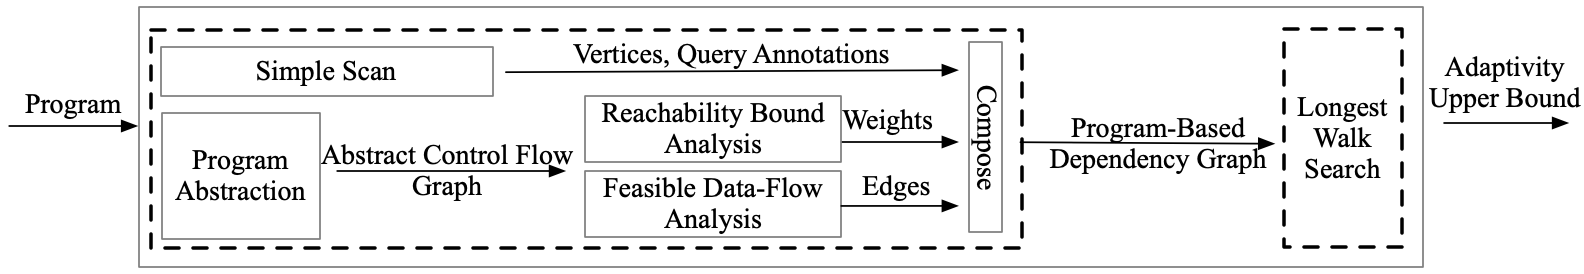
\includegraphics[width=1.0\columnwidth]{adapfun.png}
%   \vspace{-0.3cm}
%   \caption{The overview of {\THESYSTEM}}
%   \label{fig:adaptfun}
%   \vspace{-0.5cm}
% \end{figure}
%
%%%%%%%%%%%%%%%%%%%%%%%%%%%%%%%%%%% Above Previous Explanation of the Graph, for Reference  %%%%%%%%%%%%%%%%%%%%%%%%%%%%%%%%%%%%%%%
%As illustrated in Fig.~\ref{fig:adaptfun}, below is the outline of the {\THESYSTEM}.
%%%%%%%%%%%%%%%%%%%%%%%%%%%%%%%%%%% Previous Version for Reference %%%%%%%%%%%%%%%%%%%%%%%%%%%%%%%%%%%%%%%
% \textbf{1. Graph Estimation} in the double-stroke box. 
%   Because the adaptivity for a program $c$ is defined over a program's \emph{semantics-based dependency graph} (in Def.~\ref{def:trace_graph}), $\traceG(c)$,
%   this algorithm first estimates this graph statically
%   in Section~\ref{sec:alg_graphgen}.
%   It estimates the four components of this graph and then composes them into an estimated dependency graph in the last step as follows.
% \begin{enumerate}
%   \item \textbf{Vertex and Query Annotation Estimation}
%   Vertices and query annotations in this graph are identical to them in $\traceG(c)$, which are extracted directly from the program as in Section~\ref{sec:alg_vertexgen}.
%   \item \textbf{Edge and Weight Estimation}
%   \\
%   This algorithm estimates the edges and weights for $\traceG(c)$. It combines the dependency analysis and quantitative analysis techniques summarized as follows.
% %   the control, data-flow  analysis algorithm and the loop bound inference algorithm.
% %   There are three computation steps in this algorithm.
%   \\
%   \textbf{Abstract Control Flow Graph.}
%   In order to perform these combined analysis techniques, this step first generates an \emph{abstract control flow graph} for the program $c$, $\absG(c)$ in Section~\ref{sec:abscfg}.
%   \\
%   \textbf{Edges Estimation via Combined Flow Analysis.} 
%   This step is presented in
%   Section~\ref{sec:alg_edgegen}. It performs over the \emph{abstract control flow graph}, and combines the control flow and data flow analysis techniques.
%   It estimates our \emph{variable may-dependency} between each pair of the labeled variables in a program by considering both the control flow and data flow.
%   Then it uses the estimated dependency relation to approximate the edge
%   between each pair of vertices.
%   \\
%   \textbf{Weights Estimation via Quantitative Analysis.} 
%   This step is presented in Section~\ref{sec:alg_weightgen}. 
%   It performs over the same \emph{abstract control flow graph}, $\absG(c)$ and computes the upper bound on the maximal visiting times of each labeled variable for a program.
%   It estimates the reachability bound for every vertex over the  $\absG(c)$,
%   and this reachability bound is used to estimate the maximal visiting times of each labeled variable in a program and the weight of the corresponding vertex.
% \item  \textbf{Graph Estimation.} 
% In Section~\ref{sec:alg_graphgen}, we construct the final approximated graph,
% named \emph{estimated dependency graph}, $\progG(c)$ by simply composing the four estimated ingredients. 
% Overall, this \emph{estimated dependency graph} has a similar topology structure as 
% the \emph{semantics-based dependency graph}. It has the same
% vertices and query annotations, but approximated edges and weights. 
% \end{enumerate}
%%%%%%%%%%%%%%%%%%%%%%%%%%%%%%%%%%% Previous Version Above %%%%%%%%%%%%%%%%%%%%%%%%%%%%%%%%%%%%%%%

%% \jl{
%% \textbf{1. Graph Estimation}
%% % in the double-stroke box. 
%% %   Because the adaptivity for a program $c$ is defined over a program's \emph{semantics-based dependency graph} (in Def.~\ref{def:trace_graph}), $\traceG(c)$,
%% %   this algorithm first estimates this graph statically
%%   in Section~\ref{sec:alg_vertexgen} and \ref{sec:alg_weightedgegen}
%% %   It 
%%   first estimates the four components of this graph and then composes them into an estimated dependency graph in the last step as follows.
%% \begin{enumerate}
%%   \item \textbf{Vertex and Query Annotation Estimation} in Section~\ref{sec:alg_vertexgen}.
%% }

%\textbf{2. Adaptivity Computation} in Section~\ref{sec:alg_adaptcompute} computes sound bound on adaptivity over $\progG(c)$.
% Likewise the adaptivity in Def.~\ref{def:trace_adapt},
% %  is defined as a finite walk in the \emph{semantics-based dependency graph}, 
% the static estimation on the \emph{adaptivity} also 
% relies on finding a walk in the \emph{estimated dependency graph} similar to Def.~\ref{def:trace_adapt}.  
% The construction of the stastic analysis dependency graph is of great value of showing some useful properties of the target program, such as dependency between variables, the execution upper bound of a certian command, while the key novelty is our path searching algorithm, which connects all the information we need in the static anlaysis dependency graph and provides us a sound over-estimation of adaptivity! In order to get a sound but precise upper bound,
% We discuss some challenges in finding the 'appropriate' walk in the graph, and how our algorithm leverages these challenges as
% . We present the path searching algorithm 
% in Section~\ref{sec:alg_adaptcompute}.

%
%
%%%%%%%%%%%%%%%%%%%%%%%%%%%%%%%%%%%%%%%%%%%%%%%%%%%%%%%%%%%%%%%%%%%%%%%%%%%%%%%%%%%%%%%%%%%%%%%%%%%%%%%%%%%%%%%%%%%%%%%%%%%%%%%%%%%%%%%%%%%%%%%%%%%%%%%%%%
%%%%%%%%%%%%%%%%%%%%%%%%%%%%%%%%%%%%%%%%%%%%%%%%%%%%%%%%%%%% Edge And Weight Analysis %%%%%%%%%%%%%%%%%%%%%%%%%%%%%%%%%%%%%%%%%%%%%%%%%%%%%%%%%%%%%%%%
%%%%%%%%%%%%%%%%%%%%%%%%%%%%%%%%%%%%%%%%%%%%%%%%%%%%%%%%%%%%%%%%%%%%%%%%%%%%%%%%%%%%%%%%%%%%%%%%%%%%%%%%%%%%%%%%%%%%%%%%%%%%%%%%%%%%%%%%%%%%%%%%%%%%%%%%%%
%
Given a program $c$, the set of vertices $\progV(c)$ and query annotations $\progF(c)$ of the \emph{estimated dependency graph} can be computed by simply
scanning the program $c$. These set can be computed precisely and correspond to
the same sets in the semantics-based dependency graph.
This means that $\progG(c)$ has the same underlying vertex structure as 
the semantics-based graph $\traceG(c)$. The differences will be in the sets of edges and weights. 



\subsection{Weight and Edge Estimation}
\label{sec:alg_weightedgegen}
The set of edges $\progE(c)$ and the set of weights $\progW(c)$ of the estimated dependency graph are estimated through an analysis combining control flow, data flow, and loop bound analysis. These analyses are naturally described over an  \emph{Abstract Transition Graph} of the input program, which we describe next.
%
%%%%%%%%%%%%%%%%%%%%%%%%%%%%%%%%%%%%%%%%%%%%%%%%%%%%%%%%%%%% Abstract Dependency Graph %%%%%%%%%%%%%%%%%%%%%%%%%%%%%%%%%%%%%%%%%%%%%%%%%%%%%%%%%%%%%%%%
%
\subsubsection{Abstract Transition Graph}
\label{sec:abscfg}
%%%%%%%%%%%%%%%%%%%%%%%%%%%%%%%%%%%%%%%%%%%%%% Previous Version For Reference %%%%%%%%%%%%%%%%%%%%%%%%%%%%%%%%%%%%%%%%%%%%%%
% An \emph{Abstract Transition Graph}, $\absG(c)$ for a program $c$ is composed of
% a vertex set $\absV(c)$ and an edge set $\absE(c)$, $\absG(c) \triangleq (\absV(c), \absE(c))$.
% \\
% Every 
% vertex $l \in \absV(c)$ is the label of a labeled command in $c$, which is unique.
% \\
% Each edge $(l \xrightarrow{dc} l') \in \absE(c)$ is an abstract transition
% between two program points $l, l'$. 
% There is an edge from $l$ to $l'$ if and only if
% the command with label $l'$ can execute right after the execution of the command with label $l$.
% % if and only if there is a control flow between two program points.
% Each edge is annotated by a constraint $dc \in \dcdom^{\top}$, which is generated from the command with label $l$.
% This constraint describes the abstract execution of the command with $l$. 
% The edge set is constructed in three steps summarized as follows (with detail in Apdix.).
% \begin{enumerate}
%     \item Computing \textbf{constrains} over the expression for every program's labeled command,
%   which is used as the annotation of an edge.
%   Its domain $\dcdom^{\top}$ is composed of the \emph{Difference Constraints} $DC(\mathcal{VAR}  \cup \constdom)$, the \emph{Boolean Expressions} $\booldom$ and $\top$.
% %
% \begin{itemize}
% \item The difference constraints $DC(\mathcal{VAR}  \cup \constdom)$ is the set of all the inequality of
% form $x' \leq y + v$ where $x \in \mathcal{VAR} $, 
% $y \in \mathcal{VAR}$ and $v \in \constdom$.
% The \emph{Symbolic Constant} set $\constdom = \mathbb{N} \cup \inpvar \cup{\infty \cup{Q_m}}$
% is the set of natural numbers with $\infty$, the input variables, and a symbol $Q_m$ representing the abstract value of a query request.
% An inequality $x' \leq y + v$ describes that the value of $x$ in the current state is
% at most the value of $y$ in the previous state plus some constant $v$.
% When a difference constrain shows up as an edge annotation, $l \xrightarrow{x' \leq y + v} l'$,
% it denotes that
% the value of variable $x$
% after executing the command at $l$ is at most
% the value of variable $y$ plus $v$ before the execution.
% For every expression in each of the label command, it is computed in three steps via program abstraction method adopted from the Section~6 in \cite{sinn2017complexity}. 
% %
% \item The Boolean Expressions $b$ from the set $\booldom$.
% $b$ on an edge $l \xrightarrow{b} l'$ describes
% that after evaluating the guard with label $l$,
% $b$ holds and the command with label $l$ will execute right after.
% %
% \item The top constraint, $\top$ denotes true. It is preserved for $\eskip$ command.
% %
% \end{itemize}
%     \item \textbf{Initial and final state} computation step generates two sets for each labeled command in $c$. 
%   The initial state contains the
%   label where this command {starts} executing, 
%   and the final state is a set
%   that contains the constraint of this command
%   and the continuation labels after the execution of this command.
%  \item \textbf{abstract event} computation step generates a set of edges for the $c$, by computing the initial state and finial state interactively and recursively.
% \end{enumerate}
%%%%%%%%%%%%%%%%%%%%%%%%%%%%%%%%%%%%%%%%%%%%%% Previous Version Above %%%%%%%%%%%%%%%%%%%%%%%%%%%%%%%%%%%%%%%%%%%%%%
%
We say that we have a \emph{transition} from a program point $l$ to a
program point $l'$ if and only if the command with label $l'$ can
execute right after the execution of the command with label $l$.
The \emph{Abstract Transition Graph} $\absG(c)$ of a program $c$ is a
graph with the set of labels of program points in $c$  (including a 
label $\lex$ for the exit point) as the set of
vertices $\absV(c)$, and with the set of transitions in $c$ as the set of
edges $\absE(c)$. Each edge of the graph is annotated with either
the symbol $\top$, a boolean expression or a \emph{difference
constraint}~\cite{sinn2017complexity}.

A difference constraint is an inequality of the form $x' \leq y + v$ {or $x' \leq v$}
where $x, y$ are variables and $v \in \constdom$ is a symbolic
constant: either a natural number, the symbol $\infty$, an input
variable or a symbol $Q_m$ representing a query request.  We denote by
$\dcdom$ the set of difference constraints.

A difference constraint on an edge, $l \xrightarrow{x' \leq y + v}
l'$ {or $l \xrightarrow{x' \leq v} l'$}, denotes that after executing the command at location $l$ the
value of the variable $x$ is at most the value of the expression $y +
v$ {resp. $v$} before the execution of the command $l'$.
A boolean value $b$ on an
edge, $l \xrightarrow{b} l'$, denotes that after evaluating the guard
of an if or a while command with label $l$, $b$ holds and the next
command to be executed is the one with label $l'$.  A $\top$ symbol on
an edge, $l \xrightarrow{\top} l'$ denotes that the command with label
$l$ is a $\eskip$, {and the commands that do not interfere with any loop counter variable}.

We compute difference constraints and the other annotation via a
simple program abstraction method adopted
from \cite{sinn2017complexity}, described in details in the
supplementary material.
% \mg{It would be good to have a simple short sketch.}
%\\
%% \jl{   
%% 2. Computing the \textbf{Initial and final state} for each labeled command in $c$. 
%%   The initial state contains the
%%   label where this command {starts} executing, 
%%   and the final state is a set
%%   that contains the constraint of this command
%%   and the continuation labels after this command.
%%   \\ 
%% %  \item 
%% 3. computing \textbf{abstract event}s and generating a set of edges for the $c$, by computing the initial state and finial state interactively and recursively.
%% %   Each edge is a pair of initial and finial state.
%% % \end{enumerate}
%% }

\textbf{Example.}
We show in Fig.~\ref{fig:abscfg_tworound}(b) the  abstract control flow graph, $\absG(\kw{twoRounds(k)})$ of the $\kw{twoRounds(k)}$ program we gave in  Fig.~\ref{fig:overview-example}(a) and which we also report in  Fig.~\ref{fig:abscfg_tworound}(a).
% \mg{This example has many issues. First, many nodes do not respect the format that 
% we say difference constraint have. So, either we gave the wrong definition of difference constraints or we are being sloppy or we are using some shortening without telling it to the reader. In any case we need to fix this. Also, why one of the query is bound by $Q_m$ and the other one is instead bound by $k*a$? I think this example needs some serious reworking.}
% \jl{
% The edge $(1 \xrightarrow{j' \leq k} 2)$ on the top tells us the command 
% $\clabel{\assign{j}{k}}^1$ is executed with a continuation point $2$ such that the
% % where the 
% guard $\clabel{j > 0}^2$ will be evaluated next.
% The annotation $j' \leq k$ is a difference constraint 
% computed for
% % by abstracting
% the expression $k$ from the assignment command $\assign{j}{k}$.
% %  from the function $\absexpr(0)$.
% It represents that the value of $j$ is less than or equal to value of input variable $k$ after the
% execution of $\clabel{\assign{a}{0}}^0$ and before executing the loop.
% % Another example edge $5 \xrightarrow{a' \leq a + x } 2$ describes the execution of
% %  the command
% % $\clabel{\assign{a}{x + a}}^{5}$.
% The boolean constraint $j \leq 0 $ on the edge $2 \xrightarrow{j \leq 0} 6$
% represents the negation of the testing guard $j > 0$
% of the $\ewhile$ command with header at label $2$.
% }
% \mg{ The next sentence need a pass after we fix the example:
% The edge $(0 \xrightarrow{a' \leq 0} 1)$ on the top tells us the command 
% $\clabel{\assign{a}{0}}^0$ is executed with a continuation point $1$ such that the
% command $\clabel{\assign{j}{k}}^1$ will be executed next.
% % The annotation $a' \leq 0$ is a difference constraint 
% % computed for
% % the expression $0$ in the assignment command $\assign{a}{0}$.
% $a' \leq 0$ represents that the value of $a$ is less than or equal to $0$ after the
% execution of $\clabel{\assign{a}{0}}^0$ and before executing $\clabel{\assign{j}{k}}^1$.
% % Another example edge $5 \xrightarrow{a' \leq a + x } 2$ describes the execution of
% %  the command at line $5$
% % $\clabel{\assign{a}{x + a}}^{5}$.
% % This edge has difference constraint $a' \leq a+x $.
% % The $a'$ on the left side of $a' \leq a+x$ represents the value of $a$ after executing this assignment command.
% $j \leq 0 $ on the edge $2 \xrightarrow{j \leq 0} 6$
% represents the negation of the testing guard $j > 0$
% of the $\ewhile$ command with header at label $2$.
% The edge from $3$ to $4$ comes from the query request command $\clabel{\assign{x}{\query(\chi[j])} }^{3}$.
% The constraint over this edge, $x' < Q_m$ describes after executing $\assign{x}{\query(\chi[j])}$,
% % $\clabel{\assign{x}{\query(\chi[j])} }^{3}$, 
% the query request results stored in $x$ is bounded by $Q_m$. 
% }
The edge $(0 \xrightarrow{a' \leq 0} 1)$ on the top, tells us the command 
$\clabel{\assign{a}{0}}^0$ is executed with a continuation point $1$ such that the
% where the 
command $\clabel{\assign{j}{k}}^1$ will be executed next.
The annotation $a' \leq 0$ is a difference constraint 
computed for
% by abstracting
the expression $0$ in the assignment command $\assign{a}{0}$.
%  from the function $\absexpr(0)$.
It represents that the value of $a$ is less than or equal to $0$ after the
execution of $\clabel{\assign{a}{0}}^0$ and before executing $\clabel{\assign{j}{k}}^1$.
Another example edge $5 \xrightarrow{a' \leq a + x } 2$ describes the execution of
 the command at line $5$
$\clabel{\assign{a}{x + a}}^{5}$.
This edge has difference constraint $a' \leq a+x $.
The $a'$ on the left side of $a' \leq a+x$ represents the value of $a$ after executing this assignment command.
The boolean constraint $j \leq 0 $ on the edge $2 \xrightarrow{j \leq 0} 6$
represents the negation of the testing guard $j > 0$
in the $\ewhile$ command with loop header at line $2$.
The edge from $3$ to $4$ comes from a query request command.
The constraint over this edge, $x' < Q_m$ describes after executing the query request command,
$\clabel{\assign{x}{\query(\chi[j])} }^{3}$, the query request results stored in $x$ is bounded by $Q_m$. 

\begin{figure} 
    \centering
    \begin{subfigure}{.2\textwidth}
    \begin{centering}
    {\small
    $
        \begin{array}{l}
              \clabel{ \assign{a}{0}}^{0} ;   
                \clabel{\assign{j}{k} }^{1} ; \\
                \ewhile ~ \clabel{j > 0}^{2} ~ \edo ~ \\
                \Big(
                 \clabel{\assign{x}{\query(\chi[j])} }^{3}  ; \\
                 \clabel{\assign{j}{j-1}}^{4} ;\\
                \clabel{\assign{a}{x + a}}^{5}       \Big);\\
                \clabel{\assign{l}{\query(\chi[k]*a)} }^{6}\\
            \end{array}
    $
    }
    \caption{}
    \end{centering}
    \end{subfigure}
    \begin{subfigure}{.38\textwidth}
        \begin{centering}
      \begin{tikzpicture}[scale=\textwidth/20cm,samples=200]
      \draw[] (-7, 10) circle (0pt) node{{ $0$}};
      \draw[] (0, 10) circle (0pt) node{{ $1$}};
      \draw[] (0, 7) circle (0pt) node{\textbf{$2$}};
      \draw[] (0, 4) circle (0pt) node{{ $3$}};
      \draw[] (0, 1) circle (0pt) node{{ $4$}};
      \draw[] (-7, 1) circle (0pt) node{{ $5$}};
      % Counter Variables
      \draw[] (6, 7) circle (0pt) node {\textbf{$6$}};
      \draw[] (6, 4) circle (0pt) node {{ $\lex$}};
      %
      % Control Flow Edges:
      \draw[ thick, -latex] (-6, 10)  -- node [above] {$a' \leq 0$}(-0.5, 10);
      \draw[ thick, -latex] (0, 9.5)  -- node [left] {$j' \leq k$} (0, 7.5) ;
      \draw[ thick, -latex] (0, 6.5)  -- node [right] {$j > 0$}  (0, 4.5);
      \draw[ thick, -latex] (0, 3.5)  -- node [right] {$x' \leq Q_m$} (0, 1.5) ;
      \draw[ thick, -latex] (-0.5, 1)  -- node [above] {$j' \leq j - 1$} (-6, 1) ;
      \draw[ thick, -latex] (-6, 1.5)  -- node [left] {$a' \leq x + a$} (-0.5, 7)  ;
      \draw[ thick, -latex] (0.5, 7)  -- node [above] {$ j \leq 0 $}  (5.5, 7);
      \draw[ thick, -latex] (6, 6.5)  -- node [right] {$l' \leq k * a$} (6, 4.5) ;
      \end{tikzpicture}
      \caption{}
        \end{centering}
        \end{subfigure}
        \begin{subfigure}{.38\textwidth}
          \begin{centering}
        %   \todo{abstract-cfg for two round}
        \begin{tikzpicture}[scale=\textwidth/20cm,samples=200]
        \draw[] (-10, 10) circle (0pt) node{{ $0: 1$}};
        \draw[] (0, 10) circle (0pt) node{{ $1: 1$}};
        \draw[] (0, 7) circle (0pt) node{\textbf{$2: k$}};
        \draw[] (0, 4) circle (0pt) node{{ $3: k$}};
        \draw[] (0, 1) circle (0pt) node{{ $4: k$}};
        \draw[] (-10, 1) circle (0pt) node{{ $5: k$}};
        % Counter Variables
        \draw[] (6, 7) circle (0pt) node {\textbf{$6: 1$}};
        \draw[] (6, 4) circle (0pt) node {{ $\lex: 1$}};
        %
        % Control Flow Edges:
      \draw[ thick, -latex] (-8, 10)  -- node [above] {$a' \leq 0$}(-1.5, 10);
      \draw[ thick, -latex] (0, 9.5)  -- node [left] {$j' \leq k$} (0, 7.5) ;
      \draw[ thick, -latex] (0, 6.5)  -- node [right] {$j > 0 $}  (0, 4.5);
      \draw[ thick, -latex] (0, 3.5)  -- node [right] {$x' \leq Q_m$} (0, 1.5) ;
      \draw[ thick, -latex] (-1.5, 1)  -- node [above] {$j' \leq j - 1$} (-8, 1) ;
      \draw[ thick, -latex] (-8, 1.5)  -- node [left] {$a' \leq x + a$} (-1.5, 7)  ;
      \draw[ thick, -latex] (1.5, 7)  -- node [above] {$j \leq 0 $}  (4.5, 7);
      \draw[ thick, -latex] (6, 6.5)  -- node [right] {$l' \leq k * a$} (6, 4.5) ;
        \end{tikzpicture}
        \caption{}
          \end{centering}
          \end{subfigure}
      \caption{(a) The same $\kw{towRounds(k)}$ program as Figure~\ref{fig:overview-example}
      (b) The abstract control flow graph for $\kw{towRounds(k)}$  (c) The abstract control flow graph with the reachability bound for $\kw{towRounds(k)}$.}
      \label{fig:abscfg_tworound}
    \end{figure}
%

\subsubsection{Edge Estimation}
\label{sec:alg_edgegen}
The set of edges $\progE(c)$ is estimated through a combined data and control flow analysis with three components.

\noindent\textbf{Reaching definition analysis:} 
{The first component is a reaching definition analysis computing for each label $l$ in the graph $\absG(c)$ the set of labeled variables that may reach $l$ as follows.}
% \mg{Can we sketch how this analysis is performed?}
% \todo{I shortened, can you double check}
\\
{
(1). 
% For each label $l$, generating two sets of labeled variables
% % $gen(l)$, $kill(l)$ 
% where they are newly generated or destroyed by command $l$,
% \\
For each label $l$, the analysis generates two initial sets of labeled variables, $in$ and $out$, 
containing all the labeled variables $x^l$ that are newly generated but not yet reassigned before and after executing the command $l$.
\\
(2). The analysis iterates over $\absG(c)$, and updates $in(l)$ and $out(l)$ until they  are stable.
The final $in(l)$ is the set of reaching definitions $\live(l, c)$ for $l$.}
    
\noindent\textbf{Feasible data-flow analysis:} The second component is a \textbf{feasible data-flow analysis} computing for every pair $x^i, y^j \in \lvar(c)$ whether there is a flow from $x^i$ to $y^j$. This analysis is based on a relation $\flowsto(x^i, y^j, c)$ built over the sets $\live(l, c)$ for every location $l$. This relation is defined  as:
\begin{defn}[Feasible Data-Flow]
  \label{def:feasible_flowsto}
  Given a program $c$ and two labeled variables $x^i, y^j$  in this program, 
  $\flowsto(x^i, y^j, c)$ is 
  \\
    {\footnotesize
% \begin{center}
$  \begin{array}{ll}
    \flowsto(x^i, y^j, \clabel{\assign{y}{\expr}}{}^l)  & \triangleq (x^i, y^j) \in \{ (x^i, y^l) | x \in \mathsf{FV}(\expr) 
    \land x^i \in \live(l, \clabel{\assign{y}{\expr}}^l) \}  \\
    \flowsto(x^i, y^j, \clabel{\assign{y}{\query(\qexpr)}}{}^l)  & \triangleq (x^i, y^j) \in \{ (x^i, y^l) | x \in \mathsf{FV}(\qexpr) 
    % \land (y,i) \in \live(l,\clabel{\assign{x}{\query(\qexpr)}}^l) \}  \\
    \land x^i \in \live(l,\clabel{\assign{y}{\query(\qexpr)}}^l) \}  \\
    \flowsto(x^i, y^j, [\eskip]^{l})  & = \emptyset \\
    \flowsto(x^i, y^j, \eif ([b]^l, c_1, c_2))  & \triangleq \flowsto(x^i, y^j, c_1) \lor \flowsto(x^i, y^j, c_2) \\ 
        & \lor (x^i, y^j) \in
        \left\{(x^i,y^j) | x \in \mathsf{FV}(b) \land 
      %  (x,i) 
      x^i \in \live(l, \eif ([b]^l, c_1, c_2)) \land  y^j \in \lvar(c_1) \right\} \\
    %   ([y = \_]^j) \in \mathsf{blk}(c_1) \} \\
       &\lor (x^i, y^j) \in \left\{(x^i,y^j) | x \in \mathsf{FV}(b) \land 
      %  (x,i) 
      x^i\in \live(l, \eif ([b]^l, c_1, c_2))  \land  y^j \in \lvar(c_2)  \right\} \\
    %   \land ([y = \_]^j) \in \mathsf{blk}(c_2) \} \\
       \flowsto(x^i, y^j, \ewhile [b]^l \edo c_w)  & \triangleq  \flowsto(x^i, y^j, c_w)  \lor
       \\ & 
       (x^i, y^j) \in  \left\{(x^i,y^j) | x \in \mathsf{FV}(b) \land 
      %  (x,i) 
      x^i \in \live(l,   \ewhile [b]^l \edo c_w) \land  y^j \in \lvar(c_w) \right\} \\
    %   ([y = \_]^j) \in \mathsf{blk}(c_w) \} \\
       \flowsto(x^i, y^j, c_1 ;c_2)  & \triangleq \flowsto(x^i, y^j, c_1) \lor \flowsto(x^i, y^j, c_2) \\
   \end{array}$
% \end{center}
   }
   \end{defn}
This relation gives us an overapproximation of the \emph{variable may-dependency} relation for direct dependencies (dependencies that do not go through other variables).
%\jl{The transitivity of $\flowsto$ relation is a sound approximation of the $\vardep$ relation over the same pair of labeled variables.
% , in Appendix C in supplementary material
% \begin{thm}[$\vardep$ implies $\flowsto$]
% \label{thm:flowsto_soundness}
% Given a program ${c}$, for all  $ x^i, y^j \in \lvar_{{c}}$, if $\vardep(x^i, y^j, {c})$,
% then
% %  either $\flowsto(x^i, y^j, c)$ 
% % or 
% there exist $z_1^{r_1}, \cdots, z_n^{r_n} \in \lvar_{{c}}$ with $n \geq 0$ such that   
% $\flowsto(x^i,  z_1^{r_1}, c) 
% \land \cdots \land \flowsto(z_n^{r_n}, y^j, c)$
% %
% \[
% \begin{array}{l}
%   \forall x^i, y^j \in \lvar_{{c}}.
%   \vardep(x^i, y^j, {c})
%   \\ \quad \implies
%   \Big( \exists n \in \mathbb{N}, z_1^{r_1}, \cdots, z_n^{r_n} \in \lvar_{{c}} \st n \geq 0 \land
%   \flowsto(x^i,  z_1^{r_1}, c) 
%   \land \cdots \land \flowsto(z_n^{r_n}, y^j, c) \Big)
% \end{array}
% \]
% \end{thm}
%}

\noindent\textbf{Edge Construction:} The third component constructs an edge by computing a transitive closure (through other variables) of the  
 $\flowsto$ relation. There is a directed edge from  $x^i$ to $y^j$ if and only if there is chain of of variables 
    in the $\flowsto$ relation between $x^i$ and $y^j$. This is defined as follows:
   \begin{center}
$
\begin{array}{cl}
    \progE(c) \triangleq &
    % \left
    \{ 
    (y^j, x^i)  ~ \vert ~ y^j, x^i \in \progV(c)
    \land
      % \\
      \exists n, z_1^{r_1}, \ldots, z_n^{r_n} \in \lvar(c) \st 
    %   
    \\ 
    & \qquad \qquad
      n \geq 0 \land
    %   \\
      \flowsto(x^i,  z_1^{r_1}, c) 
      \land \cdots \land \flowsto(z_n^{r_n}, y^j, c) 
    % \end{array}
    % \right
    \}
    \end{array}
$
\end{center}    
% \mg{I think we should state the soundness of this analysis, at least semi-formally}
% \jl{
We prove that the set $\progE(c)$ soundly approximates the set $\traceG(c)$.
	\begin{lem}[Mapping from Egdes of $\traceG$ to $\progG$]
	\label{lem:edge_map}
	For every program $c$ we have:
   \begin{center}
$
	\begin{array}{l}
	\forall e = (v_1, v_2) \in \traceE(c)
	\st 
	\exists e' \in \progE(c) \st e' = (v_1, v_2)
	\end{array}
$
\end{center} 
	\end{lem}
% }
% by Lemma~B.2 and Theorem~C.1 in supplementary material.}
% \jl{
% 1. The \textbf{reaching definition} analysis computes a set of labeled variables, $\live(l, c)$ for every label $l$ in $c$
%   over its abstract transition graph, $\absG(c)$.
% It contains all the labeled variables reachable at label $l$. 
% \\
% 2.
% The \textbf{feasible data-flow} computation combines the $\live(l, c)$, $\absG(c)$ and data flow analysis. 
%   It computes  $\flowsto(x^i, y^j, c)$ for every pair of the $c$'s labeled variables, $x^i, y^j \in \lvar(c)$. $\flowsto(x^i, y^j, c)$ is a sound approximation 
%   of the \emph{variable may-dependency} relation, $\vardep(x^i, y^j, c)$ for every $x^i, y^j \in \lvar(c)$.
% \\
% 3. The \textbf{Edge Construction}
% is based on the $\flowsto(x^i, y^j, c)$ relation.
% There is a directed edge from the $x^i$ to $y^j$ if and only if they are in $\flowsto(x^i, y^j, c)$ relation. Soundness is in Apdix~C.
% \\
% }
% \end{enumerate} 

\textbf{Example.}
Consider Fig.~3(c),  
the edge $l^6 \to a^5$ is built by tbe$\flowsto(l^6, a^5, c)$ relation because
$a$ is used directly in the query expression $\chi[k]*a$
and we also have $a^5 \in \live(6, \kw{twoRounds(k)})$ from the reaching definition analysis.
The edge $x^3 \to j^5$  represents the control flow from $j^5$ to $x^3$, which is soundly approximated by our $\flowsto$ relation.
% \mg{We should discuss an edge that is not directly captured by flowsto. Let's just give one example that is direct flows to and one that is using transitivity.}
% \jl{
The edge $l^6 \to x^3$ is produced by the transitivity of $\flowsto(l^6, a^5, c)$ and $\flowsto(a^5, x^3, c)$. 
% }

%%%%%%%%%%%%%%%%%%%%%%%%%%%%%%%%%%%%%%%%%%%%%%%%%%%%%%%%%%%% Reachability Bound Analysis %%%%%%%%%%%%%%%%%%%%%%%%%%%%%%%%%%%%%%%%%%%%%%%%%%%%%%%%%%%%%%%%
\subsubsection{Weight Estimation}
\label{sec:alg_weightgen}
% The weight estimation algorithm performs over the same \emph{abstract control flow graph}, $\absG(c)$. 
The set $\progW(c)$ of weights for the estimated dependency graph is estimated from the Abstract Transition Graph $\absG(c)$ of $c$ using \emph{reachability-bound analysis}~\cite{GulwaniZ10}. Specifically, we estimate as the weight of a node with label $l$ a symbolic upper bounds on the execution times of the command with label $l$ obtained by reachability-bound analysis. These symbolic upper bounds are expressions with the input variables as free variables, hence they correspond to the weight functions in the semantics-based dependency graphs. 
% on the execution times of the command with label $l$ 
%and use it as the weight of the corresponding vertex $x^l \in \progV(c)$ as follows.
%

Our reachability-bound algorithm adapts to our setting ideas from previous work~\cite{ZulegerGSV11,SinnZV14,sinn2017complexity}.
Specifically, it provides an upper bound on the number of times every command can be executed by using three steps.
\begin{enumerate}
%\item For each variable $x$, this step collects three sets of edges: a) the set of edges where $x$ increases, b) the set of edges where $x$ decreases, c) the set of edges where the value of $x$ is reset to a value that doesn't depend on $x$.
\item This steps assigns to each edge  $l \xrightarrow{dc} l'\in \absE(c)$ a \emph{local bound} as follows. We look at the strongly connected components of $\absG(c)$. If the edge does not belong to any strongly connected components, then the local bound is $1$, representing the fact that the edge is not in a loop and so it get executed at most once. If the edge belongs to a strongly connected component and one of the variables $x$ in $dc$ decreases, then the local bound is $x$. Otherwise, if the edge belongs to a strongly connected component and there is a variable $y$ that decreases in the difference constraint of some other edge, and if by removing this other edge, the original edge does not belong anymore to the strongly connected components of $\absG(c)$, then the local bound is $y$. Otherwise, the local bound is $\infty$. Notice that the output is either a symbolic constant in $\constdom$ or a variable that is not an input variable.
% assigns a local bound $c$ ($c \in \constdom \cup \mathcal{V}$), if $c$ decreases in $dc$.
  
\item This step aims at determining the \emph{reachability-bound} $\absclr(e, c)$ of every edge $e\in \progE(c)$. Every bound is a symbolic expression built out of symbols in $\constdom$ and the operations $+, *, \max$. For every edge, if the local bound of this edge computed at the previous step is a symbol in $\constdom$ then this is already the reachability-bound. If instead the local bound of the edge is a variable $y$ which is not an input variable, this step will eliminate it and replace it with a symbolic expression. In order to do this, this steps will compute two quantities: first, it will recursively sum the reachability-bounds of all the edges whose difference constraint may increment the variable $y$, plus the corresponding increment; second, it will recursively sum the reachability-bounds of all the edges whose difference constraint may reset the variable $y$ to a (symbolic) expression that doesn't depend on it, multiplied by the maximal value of this symbolic expression. The sum of these two quantities provides the symbolic expression that is an upper bound on the number of times the edge can be reached. To compute these two quantities we use two mutually recursive procedures.
\end{enumerate}
Using the reachability-bound $\absclr(e, c)$ for every edge $e = (l, dc, l')$ we can provide a bound on the visiting times of each vertex $x^l \in \absV(c)$. Formally: $w = \sum\left\{  \absclr(e, c) \middle\vert e = (l, \_, \_) \right\}$.
Notice that $w$ is a symbolic arithmetic expression over symbols in $\constdom$. In particular, it may contain the input variables and so it may effectively be used as a function of the input - and capture loop bounds in terms of these inputs.
% se two steps we can construct the set of $w$ for every label $l$, as $\absW(c)$,
% % For each pair $(l, w) \in \absW(c)$, 
% where $w = \sum\left\{  \absclr(e, c) \middle\vert e = (l, \_, \_) \right\}$.
% % $\absW(c)$ is the set of pairs $(l, w)$ for every $l \in \absV(c)$.
%     % \end{enumerate}
    %
% \\
% Because the vertexes in $\absV(c)$ share the same unique label with the vertexes in $\progV(c)$,
%     we use the $w$ on the vertex $l \in \absV(c)$ directly as the weight of the vertex $x^l$ in $\progV(c)$.
%     \highlight{
% \begin{center}
%     $\progW(c) \triangleq
% %   \left
%   \{ (x^l, w)
% \mid
% x^l \in \progV(c) \land (l, w) \in \absW(c)
% \}.
%    $
% \end{center}
% }
% We prove that $w$ for every $x^l \in \progV(c)$ is a sound upper bound of its visiting times in Apdix.~D.
% w.r.t. an arbitrary initial trace $\trace_0\in \mathcal{T}_0(c)$.
 
 \begin{thm}[Soundness of the Reachability Bounds Estimation]
    \label{thm:addweight_soundness}
  Let  ${c}$ be a program and $\progW(c)$ be its estimated weight set.
  Then, for each $(x^l, w) \in \progW(c),\vtrace_0 \in \mathcal{T}_0(c), \trace \in \mathcal{T},
  v \in \mathbb{N}$ we have:
    %
  \[
   \text{ if }
  \config{{c}, \trace_0} \to^{*} \config{\eskip, \trace_0 \tracecat\vtrace} 
  \land 
  \config{\vtrace_0, w} \earrow v
  \land
  % \right\} 
  \text{ then }
  \vcounter(\vtrace, l) \leq v
  \]
  \end{thm}
Notice that in this theorem, the evaluation $\config{\vtrace_0, w} \earrow v$ is needed in order to obtain a concrete value $v$ from the symbolic weight $w$ by specifying a value for the input variables through $\vtrace_0$.

%
\textbf{Example.} 
Consider again
Fig.~\ref{fig:overview-example}(c),
the estimated weight for $a^5$ is $k$, and this is a sound estimation.
% in estimated dependency Graph as $k$ as well.
For an arbitrary $\trace_0 \in \mathcal{T}_0(c)$, we know that $\config{\trace_0, k} \earrow \env(\trace_0) k$ and
by the weight $w_k$ for the vertex $a^5$ (as in Figure~\ref{fig:overview-example}(b)) we know 
$w_k(\trace_0) = \env(\trace_0) k$. 
%
% for the rest weights' computation.
%
% \subsubsection{Dependency Graph Computation}
%    \label{sec:alg_graphgen}
% With the four components $\progV(c), \progE(c), \progW(c)$, and $\progF(c)$
% computed in each steps above, this step simply combines the four components
% % into the quantitative dependency graph for program $c$ 
% as follows,
% %
% % \\
% \highlight{
% \begin{center}
%     $
%     \progG(c) = (\progV(c), \progE(c), \progW(c), \progF(c)).
%    $
% \end{center}
% }
% Overall, $\progG(c)$ has a similar topology structure as 
% the $\traceG(c)$, differs only in edges and weights. 
%We prove that this graph is a sound approximation of $\traceG(c)$ in Apdix~B.
\subsection{Adaptivity Upper Bound Computation}
\label{sec:alg_adaptcompute}
We estimate the adaptivity upper bound, $\progA(c)$ for a program $c$ as the maximum query length over all finite walks in its \emph{estimated dependency graph}, $\progG({c})$.
%
% $\walks(\progG(c))$ represents the set of all finite walks on
%  $\progG({c})$.

\begin{defn}
[{Estimated Adaptivity}]
\label{def:prog_adapt}
{
Given a program ${c}$ and its estimated dependency graph 
$\progG({c})$
the estimated adaptivity for $c$ is 
\begin{center}
$
\progA({c})
\triangleq \max
\left\{ \qlen(k) \ \mid \  k \in \walks(\progG(c))\right \}.
$
\end{center}
}
\end{defn}

% The full definition for $\walks(\progG(c))$ and $\qlen$ over $\walks(\progG(c))$ are in the appendix.


Notice that different from a walk on $\traceG(c)$, a walk $k \in \walks(\progG(c))$ on the graph $\progG(c)$  does not rely on an initial trace. This because, similarly to what we did for the weights in $\progW(c)$ in the previous section, we use symbolic expressions over input variables. Similarly, the adaptivity bound $\progA(c)$ will also be a symbolic arithmetic expression over the input variables. With this symbolic expression we can prove the upper bound sound with respect to any initial trace. 

% We prove our estimated adaptivity is a sound upper bound of program's adaptivity in appendix.
%
\begin{thm}[Soundness of $\progA(c)$]
    \label{thm:sound_progadapt}
    For every program $c$, 
    its estimated adaptivity is a sound upper bound of its adaptivity.
\begin{center}
$
     \forall \trace_0 \in \mathcal{T}_{0}(c), v \in \mathbb{N}^{\infty} \st 
\config{\progA(c), \trace_0} \earrow v \implies A(c)(\trace_0) \leq v.
$
\end{center}
\end{thm}

Symbolic expressions as used in the weight  are great to express symbolic bounds but make the computation of 
a maximal walk harder. Specifically, one has to face two challenges. The first is non-termination.
A naive traversing strategy leads to non-termination
because the weight of each vertex in $\progG({c})$
is a symbolic expression containing input variables.
We could try to use a depth first search strategy
using the longest weighted path to approximate
the longest finite walk with the weight as
its visiting time. However, these approach would face the second challenge: approximation.
It would consistently and considerably over-approximate the adaptivity.

To address these two challenges we design an algorithm $\pathsearch$  combining 
% DFS and BFS algorithm 
Depth First Search and Breadth First Search.
The idea of this algorithm is to reduce the task of computing the longest walk to the task of computing local versions of the adaptivity on the maximal strongly connected components (SCC) of the graph $\progG(c)$ and then compose them into the program adaptivity. The algorithm  uses  
another algorithm $\pathsearch_{\kw{SCC}}$  recursively, in order to  find the longest walk for a strong connected component (SCC)of $\progG(c)$. The pseudocode of $\pathsearch_{\kw{SCC}}$ is given as Algorithm~\ref{alg:adaptscc}

% $\pathsearch(c, \progG(c))$ arranges the $\progG(c)$ into $\kw{SCC_1}, \cdots, \kw{SCC_n}$ and obtains the $\kw{r_{scc_i}}$ of each SCC from $\kw{\pathsearch_{SCC}(c, SCC_i)}$ algorithm in Alg.~\ref{alg:adaptscc}.
% Then $\pathsearch$ shrinks $\progG(c)$ into a DAG by reducing each SCC into a vertex with the weight equal to its $\kw{r_{scc_i}}$
% and computes its longest path as adaptivity.
%%%%%%%%%%%%%%%%%%%%%%%%%%%%%%%%%%%%%%%%%%%%%%%%%%%%%%%%%%%%%%%%%%%%%%%%%%%%%%%%%%%%%%%%%%%%%%%%%%%%%%%%%%%%%%%%%%%%%%%%%%%%%%%%%%%%%%%%%%%%%%%%%%%%%%%%%%
%%%%%%%%%%%%%%%%%%%%%%%%%%%%%%%%%%%%%%%%%%%%%%%%% INTRODUCTION OF ADAPTIVITY COMPUTATION ALGORITHM 1: Removed for Space Limitation%%%%%%%%%%%%%%%%%%%%%%%%%%%%%%%%%%
%%%%%%%%%%%%%%%%%%%%%%%%%%%%%%%%%%%%%%%%%%%%%%%%%%%%%%%%%%%%%%%%%%%%%%%%%%%%%%%%%%%%%%%%%%%%%%%%%%%%%%%%%%%%%%%%%%%%%%%%%%%%%%%%%%%%%%%%%%%%%%%%%%%%%%%%%%
% {\footnotesize 
% \begin{algorithm}
%     \caption{
%     {Adaptivity Computation Algorithm ({$\kw{\pathsearch(c, \progG(c))}$})}
%     \label{alg:adapt}
%     }
%     \begin{algorithmic}[1]
%     \REQUIRE The program $c$, 
%     Its program based dependency graph: $\progG(c) = (\vertxs, \edges, \weights, \qflag)$
%     \STATE {\bf init} 
%     $q$: empty queue;
%     $\kw{adapt}$ : the adaptivity of this graph initialize with $0$;
%     % \\
%     \STATE Find all Strong Connected Components (SCC) in $\progG(c)$: $\kw{SCC_1}, \cdots, \kw{SCC_n}, 0 \leq n \leq |\vertxs|$, 
%     \STATE {\bf for} each $\kw{SCC_i}$, compute its Adaptivity $\kw{SCC_i}$:
%     \quad $\kw{adapt_{scc}[SCC_i] = \pathsearch_{scc}(c, SCC_i)}$;
%     \STATE {\bf for} every $\kw{SCC_i}$:
%     \quad $q.append(\kw{SCC_i})$; $\kw{adapt_{tmp}} = 0$;
%     \STATE \qquad {\bf while} $q$ isn't empty:
%     \quad $\kw{s} = q.pop()$;  $\kw{adapt_{tmp}}_0= \kw{adapt_{tmp}}$;  $\kw{SCC_{max}}$; 
%     \STATE \qquad \qquad {\bf for} every 
%     different SCC, $\kw{s'}$ connected by $\kw{s}$ by a directed edge from $\kw{s}$:
%     \STATE \qquad \qquad \qquad {\bf if} $(\kw{adapt_{tmp}} < \kw{adapt_{tmp}}_0 + \kw{adapt_{scc}[s']})$:
%     \quad $\kw{adapt_{tmp}} = \kw{adapt_{tmp}}_0 + \kw{adapt_{scc}[s']}$; 
%     $\kw{SCC_{max} = s'} $;
%     \STATE \qquad \qquad \qquad $q.append(\kw{SCC_{max}})$;
%     \STATE \qquad $\kw{adapt} = \max(\kw{adapt}, \kw{adapt_{tmp}})$;    
%     \RETURN $\kw{adapt}$.
%     \end{algorithmic}
%     \end{algorithm}
% }
%%%%%%%%%%%%%%%%%%%%%%%%% INTRODUCTION OF ADAPTIVITY COMPUTATION ALGORITHM 1: %%%%%%%%%%%%%%%%%%%%%%
% The ${\pathsearch}$ and  detail introduction is in supplementary material.
%%%%%%%%%%%%%%%%%%%%%%%%% INTRODUCTION OF ADAPTIVITY COMPUTATION ALGORITHM 2: %%%%%%%%%%%%%%%%%%%%%%
{\footnotesize
\begin{algorithm}
            \caption{
            {\small Adaptivity Bound Algorithm on An SCC ({$\kw{\pathsearch_{scc}(c, SCC_i)}$})}
            \label{alg:adaptscc}
            }
            \begin{algorithmic}[1]
              \REQUIRE The program $c$, 
              A strong connected component of $\progG(c)$: $ \kw{SCC_i} = (\vertxs_i, \edges_i, \weights_i, \qflag_i)$
            \STATE {\bf init.} 
            % \\
            $\kw{r_{scc}}$: $\mathcal{A}_{\lin}$ List with initial value $0$.
            \STATE {\bf init.} 
            % \\ \qquad  
            $\kw{visited}$ : $\{0, 1\}$ List with initial value $0$;
            $\kw{r}$ : $\mathcal{A}_{\lin}$ List, initial value $\infty$;
            \\ \qquad  
            $\kw{flowcapacity}$: $\mathcal{A}_{\lin}$ List, initial value $\infty$;
            $\kw{querynum}$: INT List, initial value $\qflag_i(v)$.
            \STATE {\bf if} $|\vertxs_i| = 1$ and $|\edges_i| = 0$:
            \quad {\bf return}  $\qflag(v)$
            \STATE  {\bf def} {$\kw{dfs(G,s,visited)}$}:
            \STATE \qquad {\bf for} every vertex $v$ 
            connected by a directed edge from $s$:
            \STATE \qquad \qquad {\bf if} $\kw{visited}[v] = \efalse$:
            \STATE \qquad \qquad \qquad {$\kw{flowcapacity[v] = \min(\weights_i(v), {flowcapacity}[s])}$};
            \quad {$\kw{querynum[v] = querynum[s] + \qflag_i(v)}$};
            \STATE \qquad \qquad \qquad {$\kw{r[v] =  \max(r[v], flowcapacity[v] \times querynum[v]}) $}; 
            \STATE \qquad \qquad \qquad  $\kw{visited}[v] = 1$; %\#\{mark $v$ as visited\}
            \quad $\kw{dfs(G, v, visited)}$;
            \STATE \qquad \qquad {\bf else}: \#\{There is a cycle finished\}
            \STATE \qquad \qquad \qquad 
            {\small{$\kw{r[v] =  \max(r[v], r[s] +\min(\weights_i(v), {flowcapacity}[s]) * (querynum[s] + \qflag_i(v)))}$}};
            \STATE \qquad {\bf return}  $\kw{r[c]}$
            \STATE  {\bf for} every vertex $v$ in $\vertxs_i$:
            \STATE  \qquad initialize the $\kw{visited, r, flowcapacity, querynum}$ with the same value at line:2.
            \STATE  \qquad $\kw{r_{scc} = \max(r_{scc}, dfs(SCC_i, v, \kw{visited} ))}$;
            \RETURN  $\kw{r_{scc}}$
            \end{algorithmic}
            \end{algorithm}
}           
%%%%%%%%%%%%%%%%%%%%%%%%%%%%%%%%%%%%%%%%%%%%%% Previous Version For Reference %%%%%%%%%%%%%%%%%%%%%%%%%%%%%%%%%%%%%%%%%%%%%%
% The \emph{Adaptivity Computation Algorithm on An SCC ($\kw{\pathsearch_{scc}}$)}
% takes the program, $c$ and an SCC (a subgraph), 
%   $\kw{SCC_i}$ of
% %   a program's estimated dependency graph 
% $\progG(c)$ as input
% % to be precise, the input graph is SCC, and 
% and outputs the adaptivity local bound of $\kw{SCC_i}$. 
% If $\kw{SCC_i}$ contains only one vertex, $x^l$ without any edge, $\kw{\pathsearch_{scc}}$ returns the query annotation of $x^l$ as the adaptivity.
% If $\kw{SCC_i}$ contains at least one edge, 
% $\kw{\pathsearch_{scc}}$ has three steps:
% % in this algorithm: 
% 1. It first collects all the paths on $\kw{SCC_i}$. 2. Then it calculates the adaptivity of every path by a novel adaptivity computation method, $\kw{dfs}$. 3. The maximal adaptivity among all paths is the adaptivity of $\kw{SCC_i}$ in the end.
% By the property of SCC, when the algorithm starts to traverse from a vertex, it must go back to the same vertex.
% In this sense, the paths collected in step 1 are all simple cycles with the same starting and ending vertex. 
% The most interesting part is step 2. It recursively computes the adaptivity upper bound on the fly of paths collecting through a depth first search procedure $\kw{dfs}$ from line: 5-15.
% It designs a novel adaptivity computation method, which guarantees the visiting times of each vertex by its weight and addresses the \textbf{Approximation Challenge}.
% The guarantee is achieved by two special parameters $\kw{flowcapacity}$ and $\kw{querynum}$ and the updating operations in line:7 and line:10.
% % 
% \begin{itemize}
% \item $\kw{flowcapacity}$ is a list of arithmetic expressions $\mathcal{A}_{in}$.
% % for every vertex,
% It tracks the minimum weight
% along the path during the 
% searching procedure. For each vertex, it updates the minimum weight when the path reaches that vertex with $\infty$ as the initial value.
% % , inside a cycle\}
% \item $\kw{querynum}$ is a list of integer
% % of all the vertices, which is 
% initialized by query annotation $\qflag_i(v)$ for every vertex. 
% It tracks the total number of vertices with query annotation $1$
% % which are query vertices 
% along the path.
% \item
% % \\
% The updating operation
% during the traversal 
% (line: 7) and 
% at the end of the traverse (line: 10) is
% % in these two branches, 
% $\kw{flowcapacity[v] \times querynum[v]}$.
% % in line: 11 and line: 15 
% Because $\kw{querynum[v]}$ is the \# of the vertices with query annotation $1$ and $\kw{flowcapacity[v]}$ is the minimum weight over this path,
% this number is the accurate query length of this path. 
% It guarantees 
% the visiting times of each vertex on the path reaching a vertex $v$ is no more than 
% the maximum visiting times it can be on a qualified walk by $\kw{flowcapacity[v]}$,
% and 
% in the same time  compute the query length instead of weighted length through 
% $\kw{ querynum[v]}$.
% \end{itemize}
% %  its minimum visiting time, 
% In this way, we resolve the \textbf{Approximation Challenge} without losing the soundness, formally in Apdix..
% % ~\ref{apdx:adaptalg_soundness}.
% This step also guarantees the termination through a boolean list, $\kw{visited}$ in line:7 and line:13.
%%%%%%%%%%%%%%%%%%%%%%%%%%%%%%%%%%%%%%%%%%%%%% Previous Version Above %%%%%%%%%%%%%%%%%%%%%%%%%%%%%%%%%%%%%%%%%%%%%%


% The \emph{Adaptivity Computation Algorithm on An SCC ($\kw{\pathsearch_{scc}}$)}
This algorithm takes as input the program $c$ and a $\kw{SCC_i}$ of
$\progG(c)$, and outputs an adaptivity bound for $\kw{SCC_i}$. 
If $\kw{SCC_i}$ contains only one vertex, $x^l$ without any edge, $\kw{\pathsearch_{scc}}$ returns the query annotation of $x^l$ as the adaptivity.
If $\kw{SCC_i}$ contains at least one edge, 
$\kw{\pathsearch_{scc}}$:
\begin{enumerate}
\item first collects all the paths in $\kw{SCC_i}$; 
\item it then calculates the adaptivity of every path by the method $\kw{dfs}$; 
\item in the end, it outputs the maximal adaptivity among all paths as the adaptivity of $\kw{SCC_i}$.
\end{enumerate}
By the property of SCC, the paths collected in step 1 are all simple cycles with the same starting and ending vertex. 
Step 2 is the key step. It recursively computes the adaptivity upper bound on the fly of paths collected through a DFS procedure $\kw{dfs}$ (lines: 4-13). This procedure guarantees that the visiting times of each vertex is upper bounded by its weight, and addresses the approximation challenge,
via two special lists parameters $\kw{flowcapacity}$ and $\kw{querynum}$ (lines:7-11).
 
 
$\kw{flowcapacity}$ is a list of symbolic expressions $\mathcal{A}_{in}$ which tracks the minimum weight
when searching a path,
and updates the weight when the path reaches a certain vertex.
%
$\kw{querynum}$ is a list of integer
initialized with the value of the query annotation $\qflag_i(v)$ for every vertex. 
It tracks the total number of vertices with query annotation $1$
along the path.
%
The operation
at line: 8 and line: 11 implements the operation  $\kw{flowcapacity[v] \times querynum[v]}$.
Because $\kw{flowcapacity[v]}$ is the minimum weight over this path,
this guarantees that every vertex on the estimated walk is allowed to be visited at most $\kw{flowcapacity[v]}$, and this walk is a valid finite walk.
Then $\kw{querynum[v]}$ guarantees that $\kw{flowcapacity[v] \times querynum[v]}$ computes an accurate query length
because $\kw{querynum[v]}$ is only the number of the vertices with query annotation $1$,
giving a tight bound without losing the soundness.

\begin{thm}[Soundness of $\pathsearch$]
    \label{thm:adaptalg_soundness}
    For every program $c$, we have
\begin{center}
$
\pathsearch(\progG({c})) \geq \progA(c).
$
\end{center}
\end{thm}


% This step also guarantees the termination through a boolean list, $\kw{visited}$ in line:6 and line:9.

%%%%%%%%%%%%%%%%%%%%%%%%%%%%%%%%%%%%%%%%%%%%%% Previous Version For Reference %%%%%%%%%%%%%%%%%%%%%%%%%%%%%%%%%%%%%%%%%%%%%%
% \textbf{Example.}
% The example program in Fig.~\ref{fig:alg_adaptsearch_nestedwhile} illustrates how these special
% operations computes accurate and sound adaptivity for the program.
% $\pathsearch$ first find the SCC contains vertices $y^6$ and $x^9$, $\kw{SCC} = (\vertxs, \edges)$ where $\vertxs = \{y^6, x^9\}$ and
% $\edges = \{(y^6, y^6), (x^9, x^9), (x^9, y^6), (y^6, x^9)\}$.
% Then $\kw{\pathsearch_{SCC}(SCC, nestedW(k))}$ takes $\kw{SCC}$ as input,
% and starts run $\kw{dfs}$ from vertex $y^6$, 
% It first finds the path $y^6 \to y^6$. By updating parameters through Line:10 and 14, it computes the longest query length for this path as 
% $k$.
% As highlighted in Line:14, we do not update
% $\kw{querynum}$ and $\kw{flowcapacity}$ when we identify the simple cycle $y^6 \to y^6$.
% This improves the accuracy and still guarantees the soundness.
% Because in the following recursions, we continuously search for walks heading out from $y^6$, 
% the $\kw{flowcapacity}$ of this simple cycle does not restrict the walks going out of this vertex that do not interleave with the cycle $y^6 \to y^6$.
% However, if we keep updating the minimum weight, then we
% restrict the visiting times of vertices on a walk by
% using the minimum weight of vertices that do not on this walk.
% This leads to the unsoundness in computing adpativity.
% For example, if we update the $\kw{flowcapacity}[y^6]$ as $k$ after
% the $2$nd visit of $y^6$
% and visit $x^9$ via the walk $y^6 \to y^6 \to x^9$,
% then the $\kw{flowcapacity[k]}$ is 
% updated as $\min(k, k^2)$.
% So
% % 
% the visiting times of $x^9$ is restricted by $k$ on this walk.
% This restriction excludes the finite walk 
% $y^6 \to  \cdots \to y^6 \to x^9 \to \cdots \to y^9$ where $x^9$ is visited by $k^2$ times
% in the computation. 
% However, this finite walk is a valid walk and it has exactly the longest query length $1 + k + k^2$.
% In order to 
% In this sense, to guarantee the soundness,
% we don't update $\kw{flowcapacity}$ after $2$nd visits of a vertex.
% Line: 15 returns the adaptivity heading out from its input vertex.
% Line:16-18 applies $\kw{dfs}$ on every vertex of this SCC and 
% computes the adaptivity of this SCC by taking the maximum 
% value.%    %
%%%%%%%%%%%%%%%%%%%%%%%%%%%%%%%%%%%%%%%%%%%%%% Previous Version Above %%%%%%%%%%%%%%%%%%%%%%%%%%%%%%%%%%%%%%%%%%%%%%



%%%%%%%%%%%%%%%%%%%%%%%%%%%%%%%%%%%%%%%%%%%%%% Previous Version Below, Removed for the Page Limitation %%%%%%%%%%%%%%%%%%%%%%%%%%%%%%%%%%%%%%%%%%%%%%
% \jl{
% \textbf{Example.}
% The example program in Fig.~\ref{fig:alg_adaptsearch_nestedwhile} illustrates how these special
% operations computes accurate and sound adaptivity for the program.
% $\pathsearch$ first find the SCC contains vertices $y^6$ and $x^9$, $\kw{SCC} = (\vertxs, \edges)$ where $\vertxs = \{y^6, x^9\}$ and
% $\edges = \{(y^6, y^6), (x^9, x^9), (x^9, y^6), (y^6, x^9)\}$.
% Then $\kw{\pathsearch_{SCC}(SCC, nestedW(k))}$ runs $\kw{dfs}$ with vertex $y^6$ firstly, 
% and finds the path $y^6 \to y^6$. 
% By updating parameters through Line:8 and 11, it computes the query length for this path as $k$.
% As highlighted in Line:11, we do not update
% $\kw{querynum}$ and $\kw{flowcapacity}$ when we identify the simple cycle $y^6 \to y^6$.
% This improves the accuracy and still guarantees the soundness.
% Because in the following recursions, we continuously search for walks heading out from $y^6$, 
% the $\kw{flowcapacity}$ of $y^6 \to y^6$ does not restrict the walks going out of $y^6$ that do not interleave with this simple cycle.
% However, if we keep updating the minimum weight, we
% restrict the visiting times of vertices on all the other walks
% using the weights of vertices that do not on this walk.
% This leads to the unsoundness in computing adpativity.
% For example, if we update the $\kw{flowcapacity}[y^6]$ as $k$ after
% the $2$nd visit of $y^6$
% and visit $x^9$ via the walk $y^6 \to y^6 \to x^9$,
% then the $\kw{flowcapacity[k]}$ is 
% updated as $\min(k, k^2)$.
% So
% % 
% the visiting times of $x^9$ is restricted by $k$ on this walk, and the estimated adaptivity is only $1 + 2 * k$.
% However,  $x^9$ can be visited $k^2$ times and the longest finite walk is
% $y^6 \to  \cdots \to y^6 \to x^9 \to \cdots \to y^6 \to y^2$ where $y^6$ and $x^9$ is visited $k$ and $k^2$ times with query length $1 + k + k^2$.
% In this sense, to guarantee the soundness,
% we don't update $\kw{flowcapacity}$ after $2$nd visits of a vertex.
% Line: 15 returns the adaptivity heading out from its input vertex.
% Line:16-18 applies $\kw{dfs}$ on every vertex of this SCC and 
% computes the adaptivity of this SCC by taking the maximum 
% value.%    %
% }
